% 1977 年天津卷第 2(2) 题：圆中直径、弦与平行线
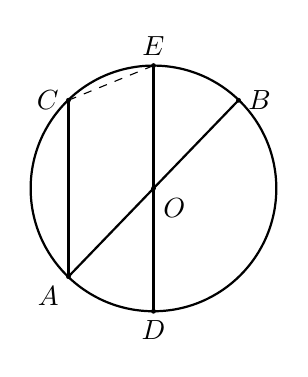
\begin{tikzpicture}[scale=0.8]
  \coordinate (O) at (0,0);
  \coordinate (A) at (-1.35,-1.4);
  \coordinate (B) at (1.35,1.4);
  \coordinate (E) at (0,1.95);
  \coordinate (D) at (0,-1.95);
  \coordinate (C) at (-1.35,1.4);
  \draw[thick] (O) circle (1.95);
  \draw[thick] (A)--(B);
  \draw[thick] (D)--(E);
  \draw[thick] (A)--(C);
  \draw[dashed] (C)--(E);
  \fill (O) circle (1.1pt) node[below right] {$O$};
  \fill (A) circle (1.1pt) node[below left] {$A$};
  \fill (B) circle (1.1pt) node[right] {$B$};
  \fill (C) circle (1.1pt) node[left] {$C$};
  \fill (D) circle (1.1pt) node[below] {$D$};
  \fill (E) circle (1.1pt) node[above] {$E$};
\end{tikzpicture}
